\section{Introduction}\label{s:introduction}

Robotics applications often require to recover the 3D shape and location of objects in world coordinates.
This explains the proliferation of datasets such as KITTI, nuScenes and SUN RGB-D~\cite{geiger12are-we-ready,nuscenes2019,sun2020scalability} which allow to train models that can classify, detect and reconstruct objects in 3D from sensors such as cameras and LiDARs.
However, creating such datasets is very expensive.
For example,~\cite{sun-rgbd,wang2019apolloscape} report that manually annotating a single object with a 3D bounding box requires approximately 100 seconds.
While this cost has since been reduced~\cite{meng2020ws3d}, it remains a significant bottleneck in data collection.

\begin{figure}[h]
    \centering
    \begin{tabular}{c c}
        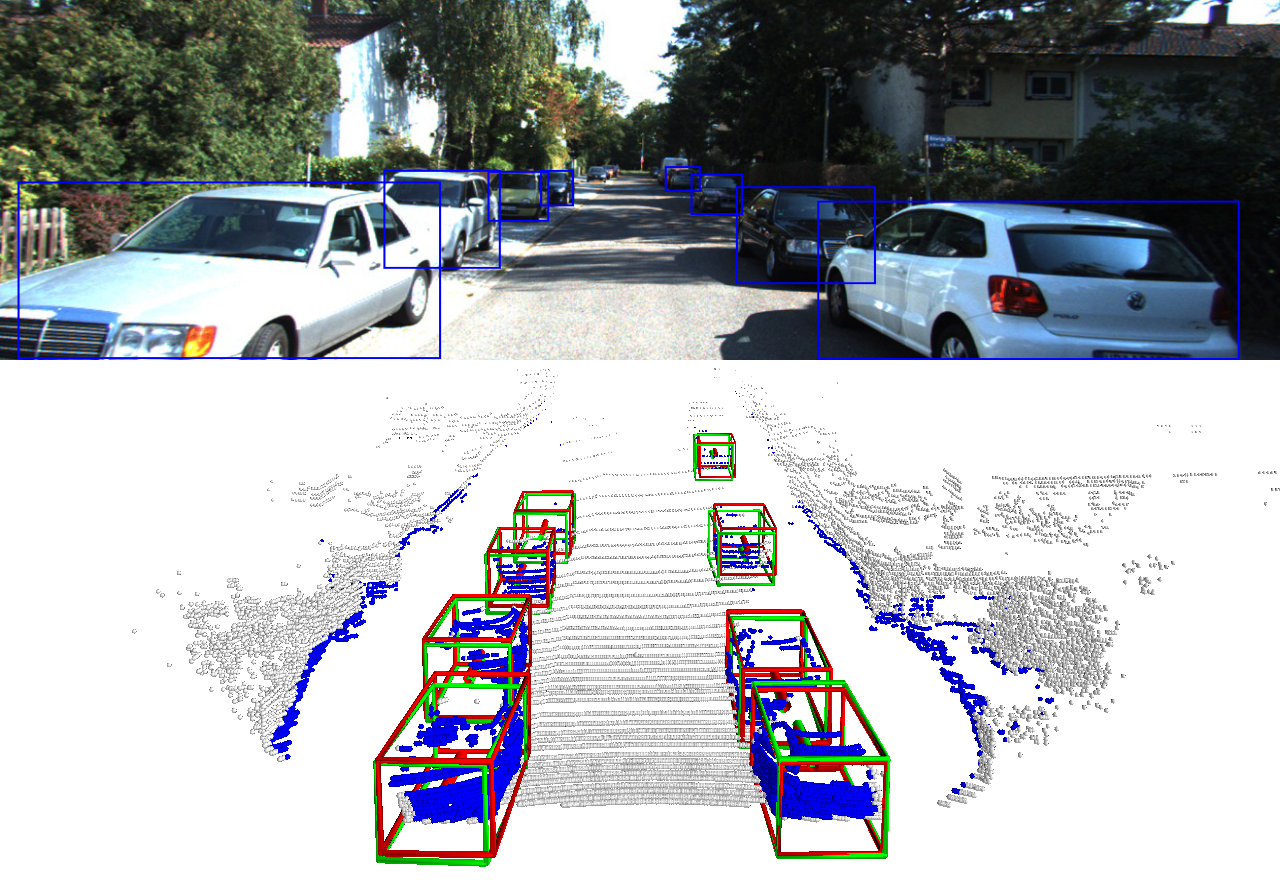
\includegraphics[width=0.5\textwidth]{figures/Qualitative_examples/411.png} & 
        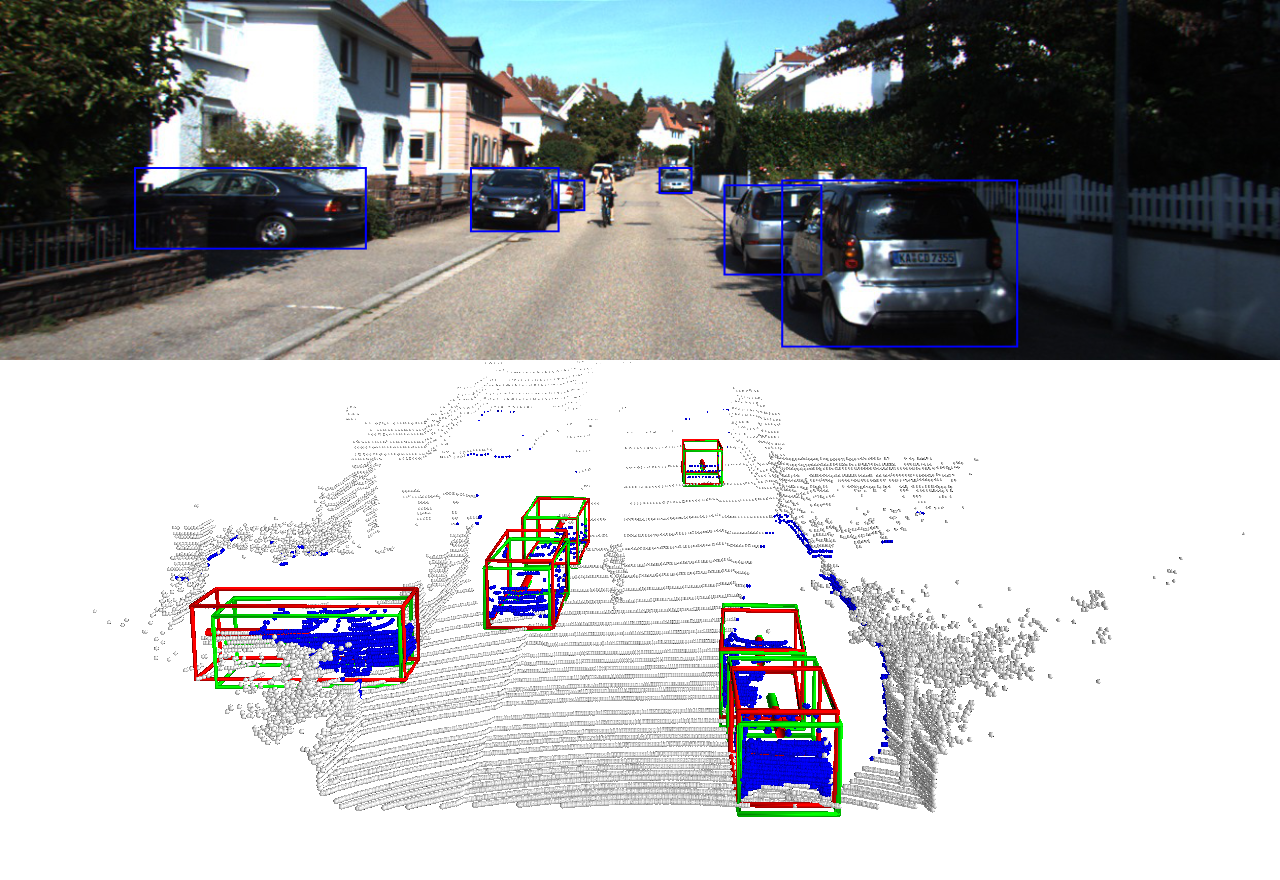
\includegraphics[width=0.5\textwidth]{figures/Qualitative_examples/50.png} \\
         
        % 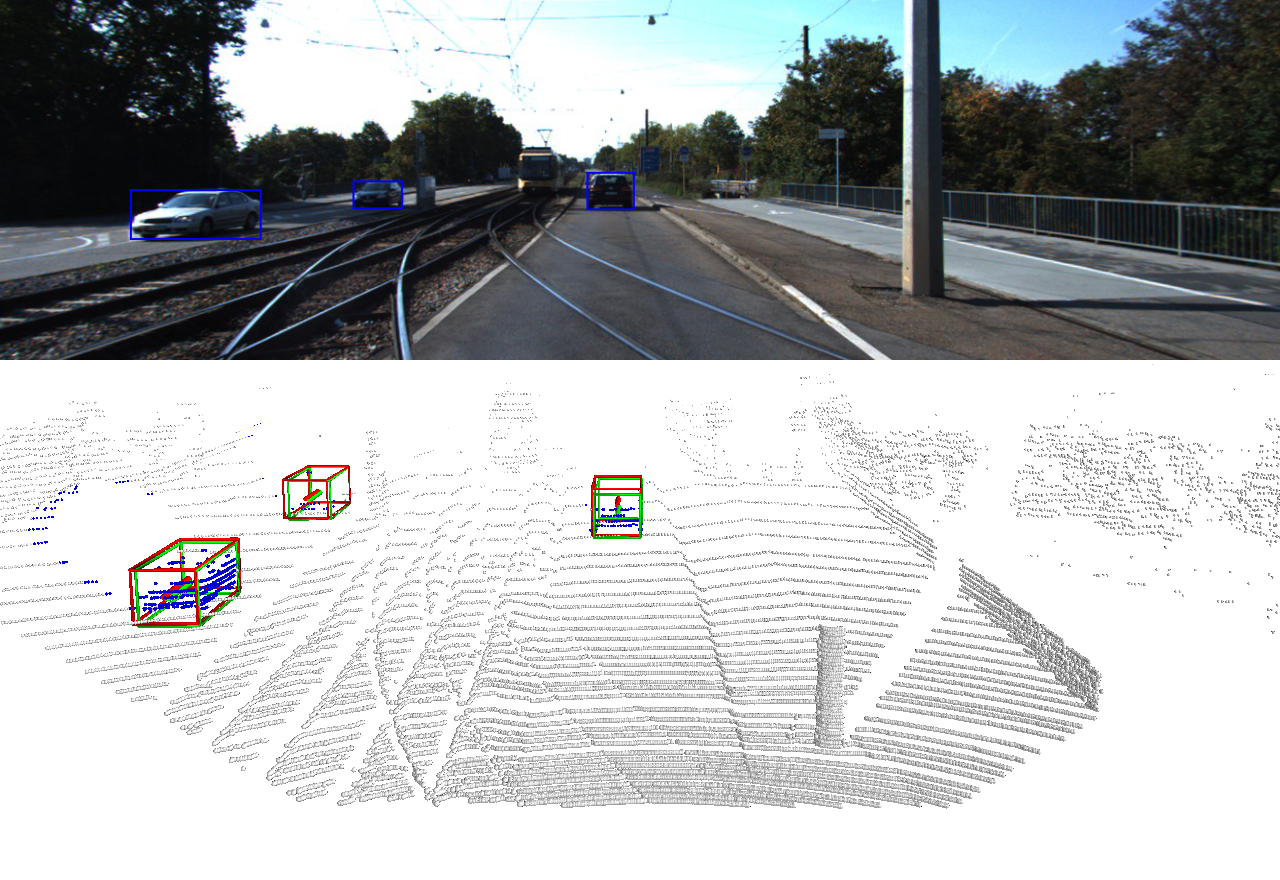
\includegraphics[width=0.5\textwidth]{figures/Qualitative_examples/172.png} & 
        % 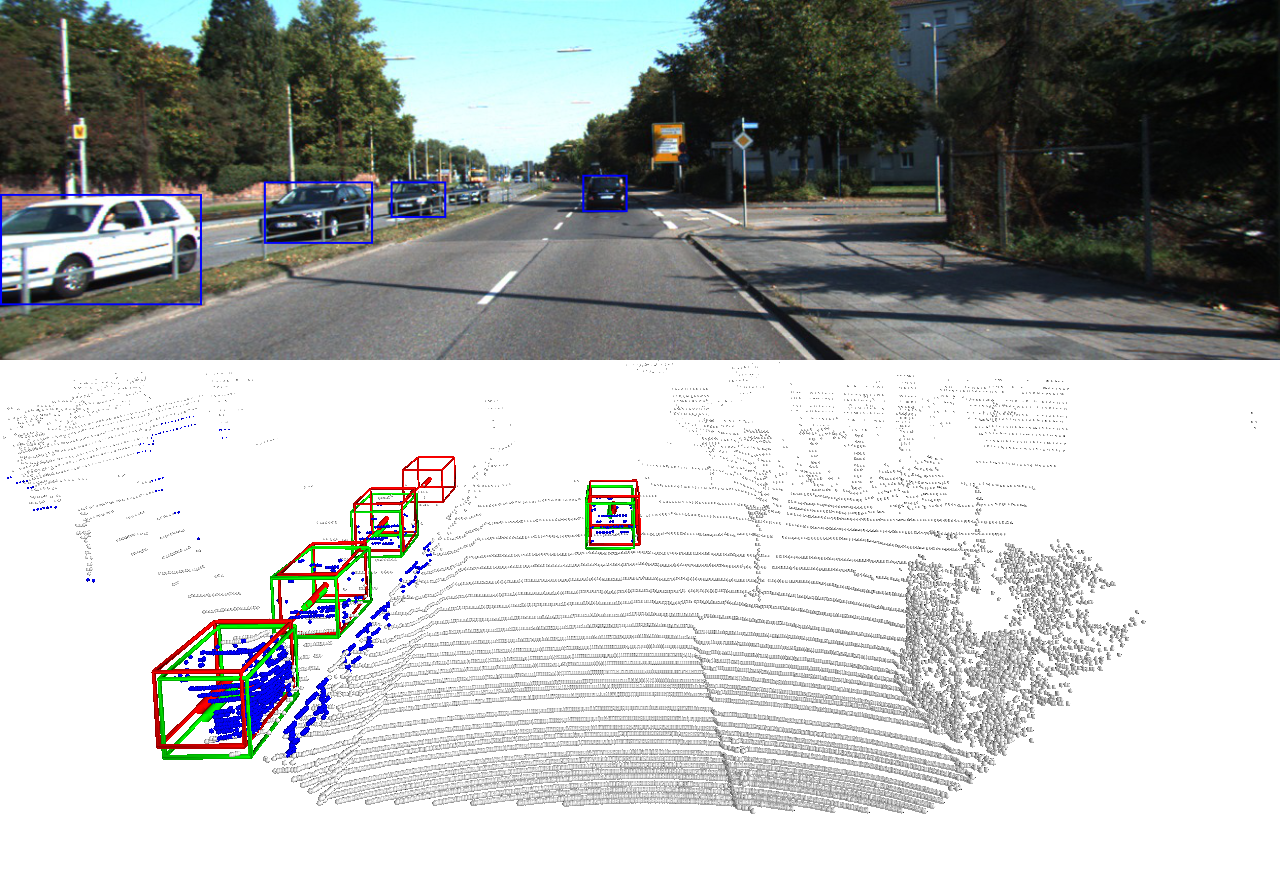
\includegraphics[width=0.5\textwidth]{figures/Qualitative_examples/52.png} \\
        
        % \includegraphics[width=0.5\textwidth]{figures/Qualitative_examples/171.png}
        %  &  \includegraphics[width=0.5\textwidth]{figures/Qualitative_examples/241.png} \\
 

        
    \end{tabular}
    \caption{Our Method (green) vs KITTI label (red), no Ground Truth is used to train our model. }
    \label{f:Qualitative}
\end{figure}
In some cases, cross-modal learning can substitute manual annotations.
% for one sensor, such as a camera, can be obtained automatically from a different sensors, such as  LiDAR\@.
An example is monocular depth prediction, where supervision from a LiDAR sensor is generally sufficient~\cite{Fu_2018_CVPR}.
Unfortunately, this does not extend to tasks such as object detection.
For instance, a dataset such as KITTI provides only $7481$ video frames annotated with objects due to the cost of manual annotation.
% LiDAR information is still used to allow annotators to determine the location of the objects in 3D space.
% However, many object occurrences are small and partially occluded, resulting in few LiDAR points per object instance and thus increasing the difficulty of obtaining correct manual annotations~\cite{feng2020labels}.
In this work, we thus consider the problem of detecting objects in 3D, thus also automatically annotating them in 3D, but using only standard 2D object detector trained on a generic dataset such as MS-COCO~\cite{lin2014microsoft}, which is disjoint from the task-specific dataset (in our case KITTI for 3D car detection).
We assume to have as input a collection of video frames, the corresponding LiDAR readings from the viewpoint of a moving vehicle, and the ego-motion of the vehicle.
We also assume to have a pre-trained 2D detector and segmenter such as Mask R-CNN\@ for the objects of interest (e.g., cars).
With this information, we wish to train a model which takes in raw LiDAR point cloud and outputs full 3D bounding box annotation for the detected objects without incurring any further manual annotation cost.

% As discussed above, this problem is rather challenging, but solving it can significantly reduce the data annotation cost and therefore allow to obtain richer and more representative labelled datasets for robotics applications.
% Because of the applicative potential, we are not the first to consider this challenge.
% For instance, the authors of~\cite{sdflabel} recently proposed a sophisticated approach for auto-labelling that uses a combination of differentiable rendering, synthetic pretraining, and canonical maps using a sign-distance-function (SDF) representation.
% The authors of~\cite{qin20weakly} proposes instead a method that combines an heuristic 3D bounding box proposal step and then learn to filter them to be compatible with the available 2D annotations.

There are three main challenges.
First, due to self and mutual occlusions, the LiDAR point clouds only cover part of the objects in a context dependent manner.
Second, the LiDAR readings are noisy, for example sometimes seeing through glass surfaces (windows) and sometimes not.
Third, the available 2D segmentations may not be perfectly semantically aligned with the target class (e.g., `vehicles' vs `cars'), are affected by a domain shift, and may not be perfectly geometrically with the LiDAR data, resulting in a large number of outlier 3D points arising from background objects.
%  that 3D points in the background can also be included in the estimate, significantly skewing any direct bounding box fit.

We propose an approach based on the following key ideas.
First, because the LiDAR point cloud can only cover the object partially, it is impossible to estimate the full 3D extent of the object from a single observation of it.
Instead, we share information between all predicted 3D boxes in the dataset by \emph{learning a 3D bounding box predictor from all the available data}.
%{\color{red} Learning the predictor is a means rather than an end:} the goal is to \emph{share information} between the thousands of object instances that exist in the dataset to obtain predictions that are overall consistent.
We further aid the process by injecting weak prior information in the form of a single fixed 3D mesh template of the object (an `average car'), but avoid sophisticated 3D priors employed in prior works~\cite{sdflabel,qin20weakly}.

We then introduce three improvements to the `obvious' baseline implementation of this idea.
First, we show that a key challenge in obtaining good 3D bounding boxes is to estimate correctly the yaw (rotation) of the object.
This is particularly challenging for partial point clouds as several ambiguous fits (generally up to rotations of 90 degrees) often exist.
Prior work has addressed this problem by using pre-trained yaw predictors, requiring manual annotation.
Here, we learn the predictor automatically form the available data only.
To this end, we show that mere local optimization via gradient descent works poorly;
instead, we propose to systematically explore a full range of possible rotations for each prediction, backpropagating the best choice every time.
We show that this selection process is very effective at escaping local optima and results in excellent, and automated, yaw prediction.

Second, we note that the LiDAR data contains significant outliers.
We thus propose to automatically learn the \emph{pattern} of such outliers by predicting a confidence score for each 3D point, treated as a Gaussian observation.
These confidences are self-calibrated using a neural network similar to the ones used for point cloud segmentation, configured to model the aleatoric uncertainty of the predictor.

Third, we note that we generally have at our disposal \emph{video data}, which contains significant more information than instantaneous observations.
We leverage this information by enforcing a simple form of temporal consistency across several frames.

As a result of these contributions we obtain a very effective system for automatically labelling 3D objects.
Our system is shown empirically to outperform relevant prior work by a large margin, all the while being simpler, because it uses less sources of supervision and because it does \emph{not} use sophisticated prior models of the 3D objects nor a large number of 3D models as priors~\cite{sdflabel,qin20weakly}

% In this work, we suggest an alternative approach that directly lifts 2D annotations in 3D.
% Given a 2D bounding box annotation and the corresponding object mask from Mask R-CNN, we first select the LiDAR points that fall within this region.
% This results in a noisy collection of 3D points, part of which correspond to the target object (inliers), and part to the background or other objects (outliers).
% Then, we fit to these LiDAR points to an `average' car template (a simple off-the-shelf 3D mesh) by minimizing a fitting loss, thus obtaining the location of the object in 3D.

% While this simplistic approach fails to generate satisfactory results, we introduce two ideas that substantially improve its performance.
% The first idea is to avoid minimizing the fitting loss directly;
% instead, we learn a neural network that, given a point cloud as input, produces as output the parameters of the fit.
% Since this network is trained using the same fitting loss and data samples as before, it is not immediately obvious why this should bring any benefits.
% The reason, we show, is that the network can pool information across \emph{all} object instances in the dataset in order to fit each individual instance.
% In other words, by observing the samples collection as a whole, the network extracts a data prior.
% By leveraging this prior, it can obtain much better fits for those object instances for which the LiDAR evidence is noisy, ambiguous or scarce.

% A second significant issue is the presence of outliers in the data.
% For the most part, outliers are LiDAR points that are incorrectly assigned to the target object due to imperfections in the Mask R-CNN detection.
% This is particularly serious when, as it is often the case, several objects partially overlap, because the algorithm may just decide to fit the incorrect object instance.
% We address this issue by extending our fitting network with the ability to predict a confidence that individual LiDAR points are inliners with respect to the selected target object.
% We cast this as a probabilistic observation model, and task the network to predict a per-point fitting variance.
% The resulting probabilistic loss function is self-calibrated and effectively learns to distinguish inliers from outlier.

% We show empirically that our approach is considerably simpler than~\cite{sdflabel}, while achieving superior accuracy.

